\section{题面结构与几何背景}

本题以假目标为坐标原点，导弹均朝假目标飞行，真目标位于 \(y=200\,\mathrm{m}\) 附近。为了避免后续模型只堆公式而缺少空间解释，先给出导弹、无人机和目标的平面位置示意，如图 \ref{fig:problem-overview-xy} 所示。图中箭头表示导弹朝假目标方向飞行，真目标投影仅作示意放大。

\begin{figure}[htbp]
  \centering
  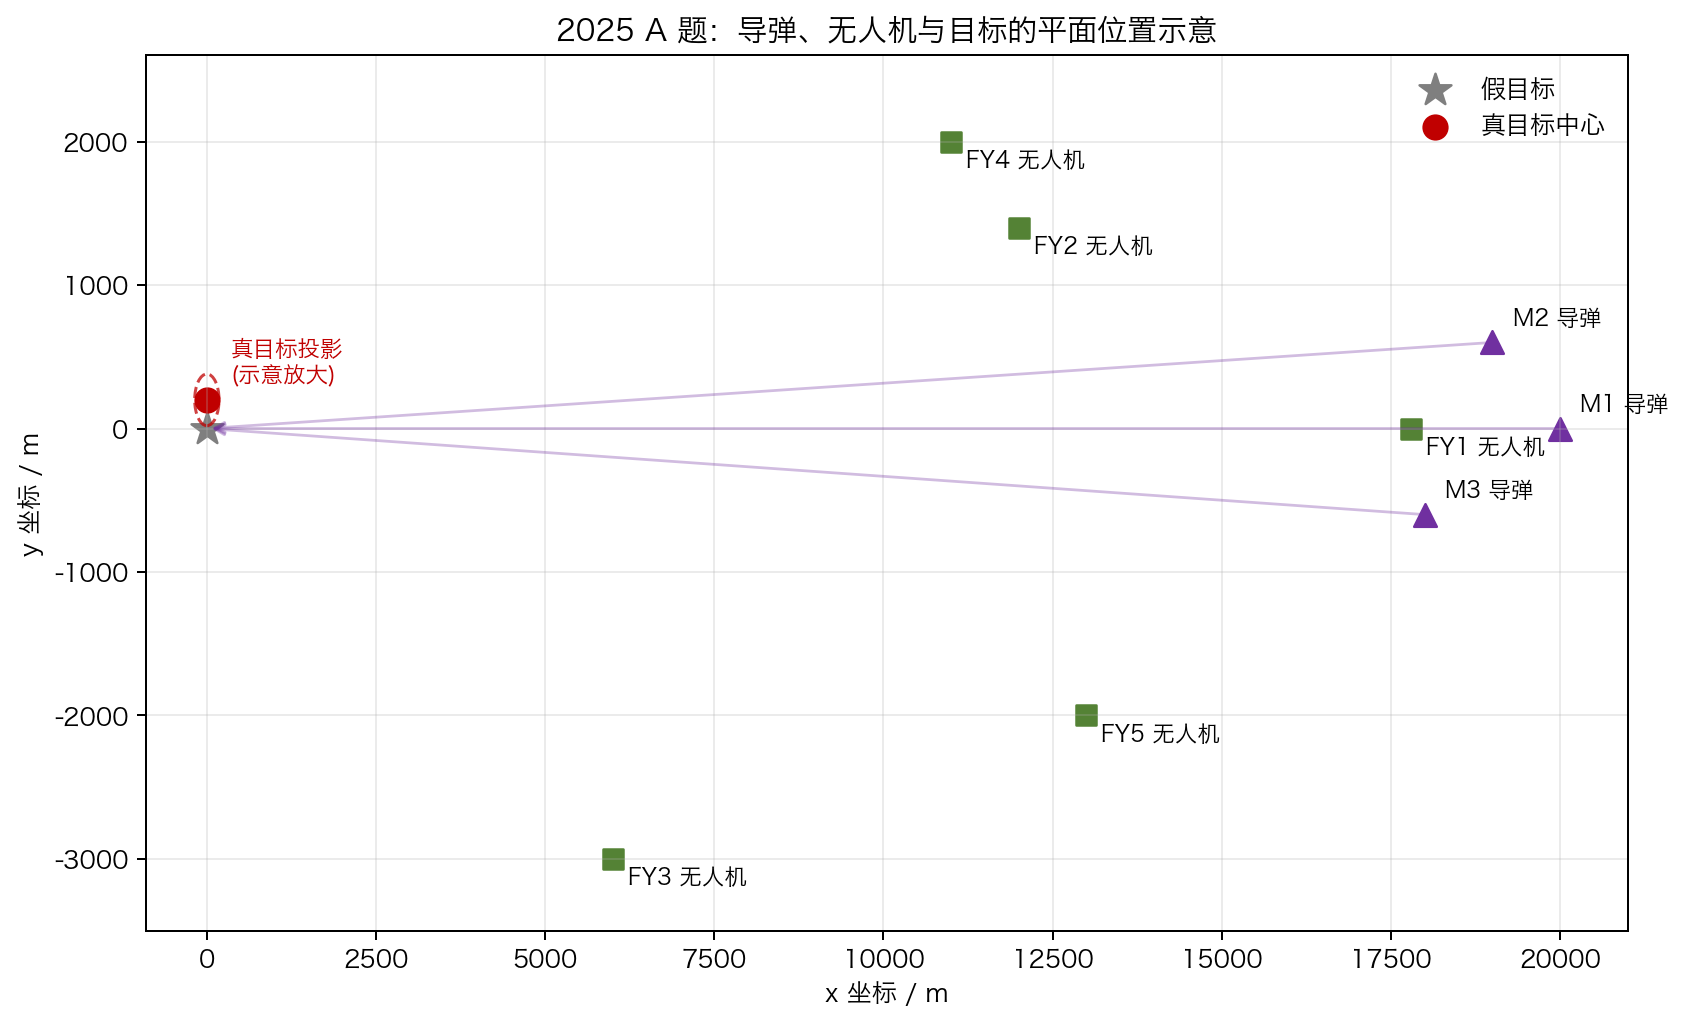
\includegraphics[width=0.92\linewidth]{../figures/fig_problem_overview_xy.png}
  \caption{2025 A 题导弹、无人机与目标的平面位置示意。该图用于说明坐标系、初始位置和来袭方向，不作为数值求解结果。}
  \label{fig:problem-overview-xy}
\end{figure}

五个子问题逐步从单机单弹扩展到多机多弹多导弹，资源范围和输出要求如图 \ref{fig:problem-question-scope} 所示。后续求解按子问题分别保存代码、表格、图和结果注册记录，避免不同问题的策略变量混用。

\begin{figure}[htbp]
  \centering
  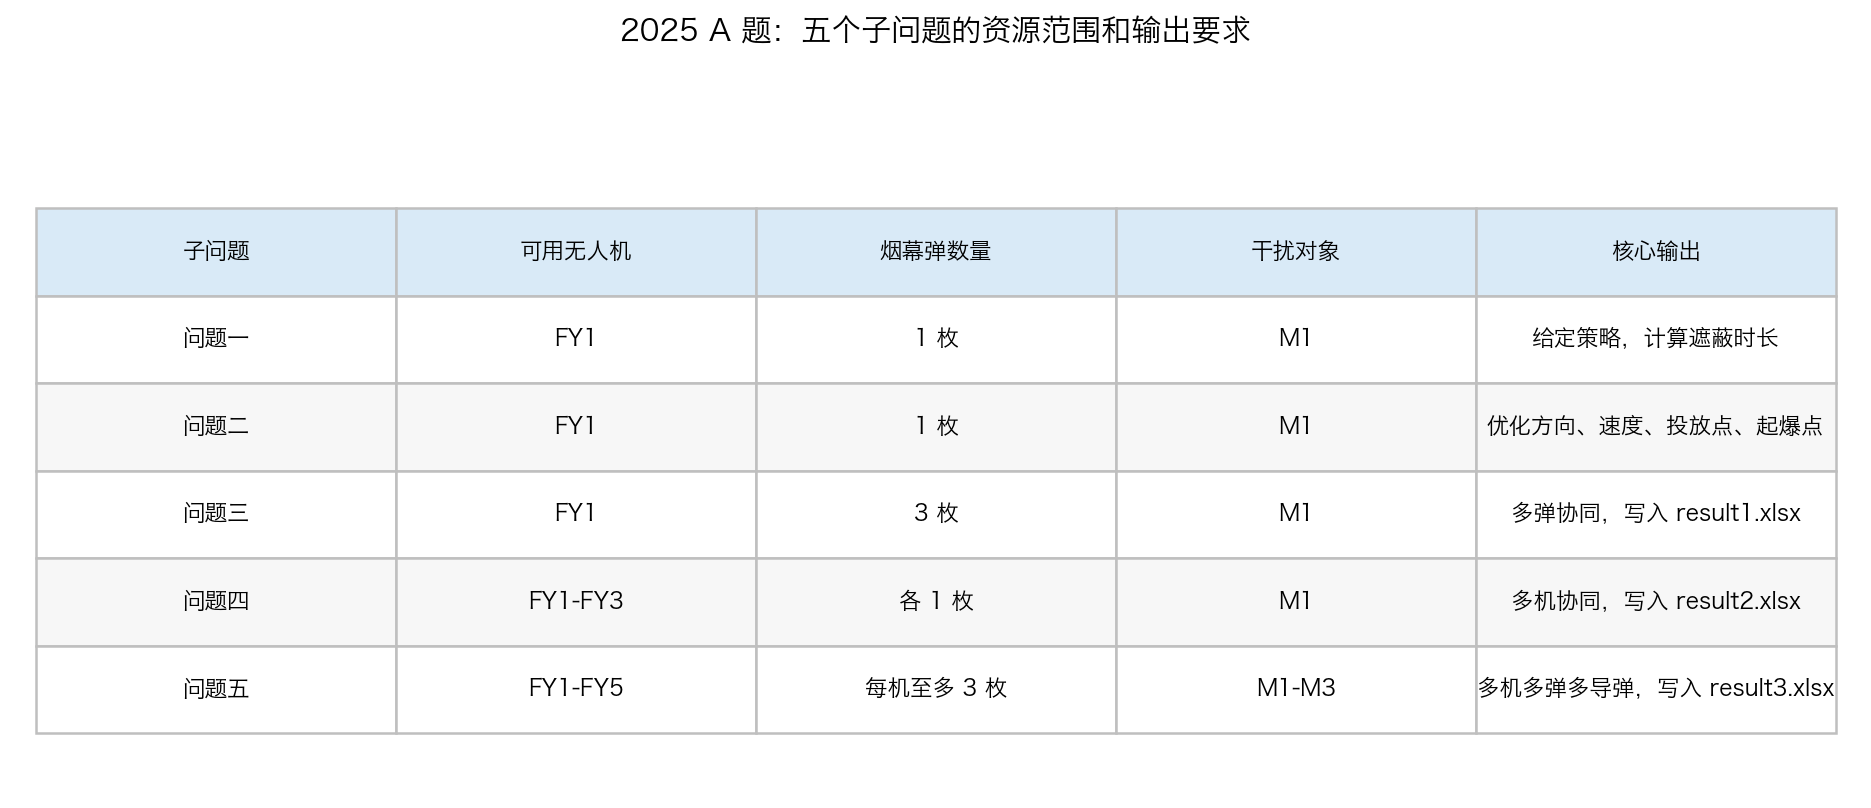
\includegraphics[width=0.94\linewidth]{../figures/fig_problem_question_scope.png}
  \caption{2025 A 题五个子问题的资源范围和输出要求示意。该图用于说明任务拆解关系。}
  \label{fig:problem-question-scope}
\end{figure}
